\def\ReadCommandLineArg#1 {%
  \def\CommandLineArg{#1}%
  \input{\jobname}}
\unless\ifdefined\CommandLineArg
\endinput\expandafter\expandafter\expandafter\ReadCommandLineArg\fi

\documentclass[english]{book}
\usepackage[T1]{fontenc}
\usepackage[utf8]{inputenc}
\usepackage{geometry}
\geometry{verbose,tmargin=2cm,bmargin=2cm,lmargin=3cm,rmargin=2cm}
\setcounter{secnumdepth}{3}
\setcounter{tocdepth}{3}

\usepackage{ifthen}
\usepackage{graphicx}

\usepackage{float}

\usepackage[english]{babel}
\addto\captionsenglish{\renewcommand{\chaptername}{Bölüm}}
\addto\captionsenglish{\renewcommand{\contentsname}{İçindekiler}}


\begin{document}
\hyphenrules{turkish}
\title{Denemeler}
\author{Yazar Adı Soyadı}
\maketitle
%
\mainmatter
\tableofcontents
%
\ifthenelse{\equal{\CommandLineArg}{kitap}}
{
\chapter{GİRİŞ}
Bu birinci bölüme ait bilgilerdir.

\begin{figure}[H]
\centering
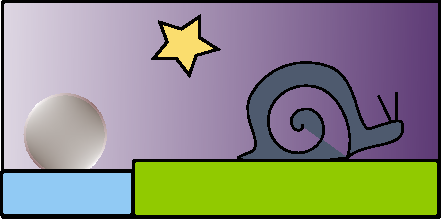
\includegraphics{chapter1/graphs/drawing}
\caption{Bu bir grafikdir}
\end{figure}


\chapter{DENEYSEL}
Bu birinci bölüme ait bilgilerdir.

\chapter{SONUÇ}
Bu birinci bölüme ait bilgilerdir.

}
{
\input{\CommandLineArg/\CommandLineArg}
}

\end{document}

